\chapter{IPFS}
\label{ipfs}

IPFS stands for InterPlanetary File System and is a peer-to-peer distributed filesystem designed to make the Web faster, safer, and more open. In contrast with standard filesystem, objects in IPFS are content-addressed by the cryptographic hash of their contents. In the case of the standard Web, when user wants some file, he needs to know on which server is a file located and the full path to the file (see figure \ref{webAddressing}). In IPFS user needs only to know the hash of the requested file. He does not care about the location of the file (see figure \ref{ipfsAddressing}). Let us take a very famous file, and add it to IPFS. Here is the plain-text MIT license:

\begin{figure}[H]
    \texttt{Permission is hereby granted, free of charge, to any person obtaining a copy of this software and associated documentation files (the "Software"), to deal in the Software without restriction, including without limitation the rights to use, copy, modify, merge, publish, distribute, sublicense, and/or sell copies of the Software, and to permit persons to whom the Software is furnished to do so, subject to the following conditions:\\\\ The above copyright notice and this permission notice shall be included in all copies or substantial portions of the Software.\\\\ THE SOFTWARE IS PROVIDED "AS IS", WITHOUT WARRANTY OF ANY KIND, EXPRESS OR IMPLIED, INCLUDING BUT NOT LIMITED TO THE WARRANTIES OF MERCHANTABILITY, FITNESS FOR A PARTICULAR PURPOSE AND NONINFRINGEMENT. IN NO EVENT SHALL THE AUTHORS OR COPYRIGHT HOLDERS BE LIABLE FOR ANY CLAIM DAMAGES OR OTHER LIABILITY, WHETHER IN AN ACTION OF CONTRACT, TORT OR OTHERWISE, ARISING FROM, OUT OF OR IN CONNECTION WITH THE SOFTWARE OR THE USE OR OTHER DEALINGS IN THE SOFTWARE.}
\end{figure}

\noindent If somebody tries to add this license as a file to IPFS, it will return \texttt{QmWpvK4bYR7k9b1feM48fsk\-t2XsZfMaPfNnFxdbhJHw7QJ} every time. That is now and will be in the future, the \textit{content address} of that file. Later, when user try to get this file by its hash, he can get it from a random person that added it into IPFS in the past.


\begin{figure}[h]
    \centering
    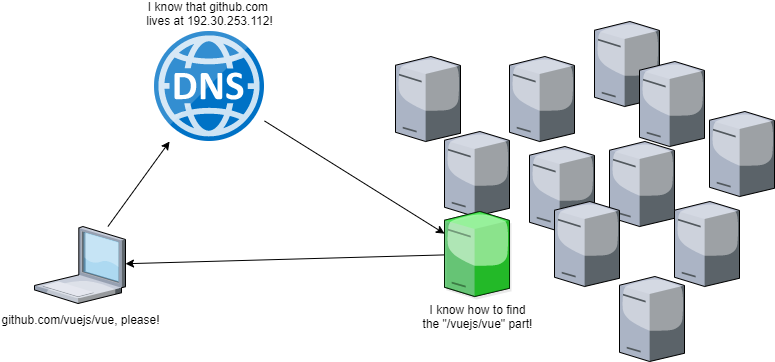
\includegraphics[width=11cm]{classicWebAddresing.png}
    \caption{Classic web addresing}
    \label{webAddressing}
\end{figure}

\begin{figure}[h]
    \centering
    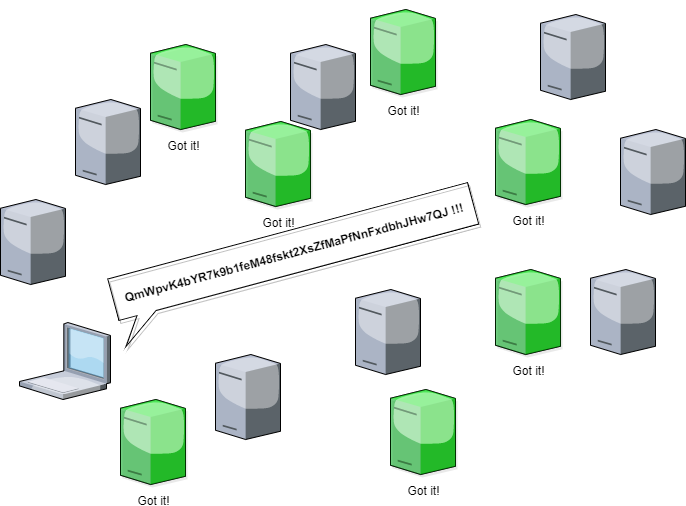
\includegraphics[width=11cm]{ipfsAddressing.png}
    \caption{Content-based addressing}
    \label{ipfsAddressing}
\end{figure}

\section{IPFS stack}
Like in other network models, we can IPFS split into layers (see figure \ref{IPFSstack}). There is \textit{libp2p}\footnote{\url{https://libp2p.io/}} at the bottom, which is peer-to-peer networking module, that handles peer and content discovery, transport, security, identity, peer routing, and messaging. \textit{IPLD} is the data model of the content-addressable web. It is providing linking between objects and multihash computing. On the top is \textit{IPFS} which allows to publish and share files (or any data).\cite{IPFSwhitepaper}


\begin{figure}[h]
    \centering
    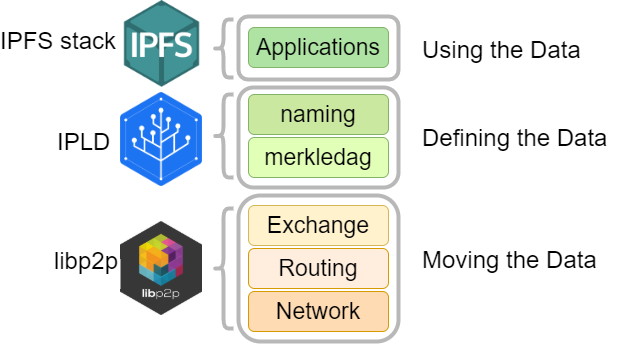
\includegraphics[width=11cm]{IPFSstack.png}
    \caption{IPFS stack}
    \label{IPFSstack}
\end{figure}


\section{libp2p}
Libp2p is transporting layer for IPFS. It grew out of IPFS to solve networking problems in p2p networks, but now it does not require or depend on IPFS. Today many projects use libp2p as their network transporting layer. For both content discovery and peer routing, libp2p uses Kademlia-based distributed hash table. With Kademlia libp2p iteratively route requests closer to the desired peer or content using Kademlia routing algorithm \cite{kademlia}. In the future, Kademlia might be changed easily to some other solutions that implement simple interface in figure \ref{libp2pInterface}.


\begin{figure}[h]
    \centering
    \begin{lstlisting}
        // gets a particular peer's network address
        FindPeer(node NodeId)

        // stores a small metadata value in DHT
        SetValue(key []bytes, value []bytes)

        // retrieves small metadata value from DHT
        GetValue(key []bytes)

        // announces this node can serve a large value
        ProvideValue(key Multihash)

        // gets a number of peers serving a large value
        FindValuePeers(key Multihash, min int)

    \end{lstlisting}
    \caption{libp2p interface}
    \label{libp2pInterface}
\end{figure}

\section{IPLD}
IPLD is providing linking and addressing objects with CID (Content ID). CID is hash-based self-describing content identifier (usually encoded to base58\footnote{\url{https://en.wikipedia.org/wiki/Base58}} format) which includes codec and multihash. Multihash is then further composed of hashtype and hash value. Let us look closer on the MIT license file, that we add to IPFS at the beginning of this chapter (see figure \ref{ipfs}). It's CID is \texttt{QmWpvK4bYR7k9b1feM48fsk\-t2XsZfMaPfNnFxdbhJHw7QJ}. It can be converted to human-readable format as can be seen in figure \ref{tab:CIDexample}, thanks to multicodec table\footnote{\url{https://github.com/multiformats/multicodec/blob/master/table.csv}}. We can see that this CID is encoded in base58 format and the file was stored using protobuf\footnote{\url{https://en.wikipedia.org/wiki/Protocol\_Buffers}} codec (this information is necessary to decode file correctly).



\begin{table}[]
    \centering
    \begin{tabular}{|ll|l|}
    \hline
    \textbf{Property}                  &             & \textbf{Value}                                                            \\ \hline
    Multibase                                        &             & base58btc                                                        \\ \hline
    Version                                          &             & cidv0                                                            \\ \hline
    Multicodec                                       &             & dag-pb                                                           \\ \hline
    \multicolumn{1}{|l|}{\multirow{3}{*}{Multihash}} & Hash Type   & sha2-256                                                         \\ \cline{2-3} 
    \multicolumn{1}{|l|}{}                           & Hash Length & 256                                                              \\ \cline{2-3} 
    \multicolumn{1}{|l|}{}                           & Hash        & 7e1b666c0327...3dc3022f \\ \hline
    \end{tabular}
    \caption{Human redable version of CID \texttt{QmWpvK4bYR7k9b1feM48fskt2XsZfMaPfNnF\-xdbhJHw7QJ}}
    \label{tab:CIDexample}
\end{table}

\section{IPFS}
IPFS is the top layer from the IPFS stack. It is used for pinning objects and files, naming system (see IPNS\footnote{\url{https://docs.ipfs.io/guides/concepts/ipns/}}) and keys management. File or object is automatically pinned when a user adds it (but other IPFS commands do not include automatic pinning). Pinning a CID tells an IPFS server that the data is important and must not be thrown away. When garbage collection is triggered on a node, any pinned content is automatically exempt from deletion. Non-pinned data may be deleted. The InterPlanetary Name System (IPNS) is a system for creating and updating mutable links to IPFS content. Since objects in IPFS are content addressed, an object's address changes every time an object's content changes. A name in IPNS is the hash of a public key. It is associated with a record containing information about the hash it links to that is signed by the corresponding private key.




\section{Existing blockchain explorers in IPFS}
In IPFS, there are already stored a few blockchains of cryptocurrencies. These blockchains are stored in raw binary format, so custom IPLD codec has to be created for every type of object. Existing codecs for cryptocurrencies are very limited. Only a few of them are currently available in IPLD (see figure  \ref{ipldFormatsCrypto}). Using custom codecs for cryptocurrencies allows explorers to request blocks and transactions by its hash very fast. Implementation and approval of new codec can take months. Existing cryptocurrency explorers build on IPFS\footnote{IPFS Zcash Blockchain explorer - \url{https://github.com/whyrusleeping/zcash-explorer}} has minimal functionality because of strict codec format. There can not be any aggregate information like transaction value in US dollars or address balance and no filtering or sorting.

\begin{table}[]
\centering
\begin{tabular}{|l|l|l|}
\hline
\textbf{Name}        & \textbf{Code} & \textbf{Description}                             \\ \hline
leofcoin-block       & 0x81          & Leofcoin Block                                   \\ \hline
leofcoin-tx          & 0x82          & Leofcoin Transaction                             \\ \hline
leofcoin-pr          & 0x83          & Leofcoin Peer Reputation                         \\ \hline
eth-block            & 0x90          & Ethereum Block (RLP)                             \\ \hline
eth-block            & 0x90          & Ethereum Block (RLP)                             \\ \hline
eth-block-list       & 0x91          & Ethereum Block List (RLP)                        \\ \hline
eth-tx-trie          & 0x92          & Ethereum Transaction Trie (Eth-Trie)             \\ \hline
eth-tx               & 0x93          & Ethereum Transaction (RLP)                       \\ \hline
eth-tx-receipt-trie  & 0x94          & Ethereum Transaction Receipt Trie (Eth-Trie)     \\ \hline
eth-tx-receipt       & 0x95          & Ethereum Transaction Receipt (RLP)               \\ \hline
eth-state-trie       & 0x96          & Ethereum State Trie (Eth-Secure-Trie)            \\ \hline
eth-account-snapshot & 0x97          & Ethereum Account Snapshot (RLP)                  \\ \hline
eth-storage-trie     & 0x98          & Ethereum Contract Storage Trie (Eth-Secure-Trie) \\ \hline
bitcoin-block        & 0xb0          & Bitcoin Block                                    \\ \hline
bitcoin-tx           & 0xb1          & Bitcoin Tx                                       \\ \hline
zcash-block          & 0xc0          & Zcash Block                                      \\ \hline
zcash-tx             & 0xc1          & Zcash Tx                                         \\ \hline
stellar-block        & 0xd0          & Stellar Block                                    \\ \hline
decred-block         & 0xe0          & Decred Block                                     \\ \hline
dash-block           & 0xf0          & Dash Block                                       \\ \hline
\end{tabular}
\caption{Existing IPLD formats for cryptocurrencies}
\label{ipldFormatsCrypto}
\end{table}